\documentclass{report}

\usepackage{color}
\usepackage{graphicx}
\graphicspath{{img_src/}}

\usepackage[left=2cm,right=2cm,top=2cm,bottom=2cm]{geometry}

\begin{document}


	\title{Cahier des charges du projet "SUPER RETRO WORLD"}
	\author{By \bsc{The Missing Part}}
	\date{\oldstylenums{2017}} 

	\tableofcontents

	\part{Historique}
		\chapter{Tracabilit\'{e}}
			\section{Versions du document actuel}
\begin{tabular}{|c|c|l|}
\hline
Versions & Date & Commentaire \\
\hline
0.1 & 20/09/17 & Cr\'{e}ation du CdC \\
\hline
0.2 & 20/09/17 & Mise à jour du chapitre "Optimisation" \\
\hline
0.3 & 20/09/17 & Mise à jour des chapitres "Description du projet" et "Exigences majeures du projet" \\
\hline
0.4 & 21/09/17 & Mise à jour du chapitre "Description du projet" \\
\hline
\end{tabular}

	\setcounter{chapter}{0}

	\part{Introduction}
	\setcounter{chapter}{0}
		\chapter{Description du projet}
			\section{Synopsis}

\paragraph{{\color{red}Un jeune robot} m\'{e}lancolique ne reçoit plus de nouvelles de son ami d’enfance. Il avait pour habitude de lui envoyer des cartes postales de ses vacances mais a subitement arrêt\'{e} de le faire il y a peu. }

\paragraph{{\color{red}Le jeune robot} parcourt souvent ces cartes en se rem\'{e}morant son ami qui ne donne plus de nouvelles. Il a construit une machine pouvant projeter ces cartes sur une grande toile afin de pouvoir ressentir la joie de voyager à travers le monde, comme son ami a toujours pu le faire.}

\paragraph{Au fil de ces cartes, {\color{red}il} se rendra compte que son ami a \'{e}t\'{e} enlev\'{e} par un être myst\'{e}rieux et continuera de parcourir le monde grâce à se machine afin de continuer son enquête.}

\paragraph{Une fois qu’{\color{red}il} aura compris qui est le kidnappeur et où il cache son ami, il s’y rendra, mais priv\'{e} de ses pouvoirs il ne pourra rien faire. Son ami d’enfance fournira alors la derni\`{e}re carte postale qu’il n’a pas pu envoyer. Cela permettra {\color{red}au jeune robot} de d\'{e}bloquer le dernier monde et de sauver son ami avant qu’il ne se fasse kidnapper.}

		\chapter{Documents relatifs et sources}
		\chapter{Objectifs}

\paragraph{L'objectif principal du projet est de proposer une exp\'{e}rience r\'{e}tro aux joueurs.}

		\chapter{Equipe de d\'{e}veloppement}

			\section{Logo}

\paragraph{Le logo doit repr\'{e}senter le potentiel de l'\'{e}quipe à pouvoir cr\'{e}er du gameplay \'{e}mergent et unique. Le but est donc d'imager l'imagination et la technique => Un cerveau dont la partie manquante viendrait d'ajouter. "The missing part" est pour l'instant le nom retenu pour l'\'{e}quipe.}


\begin{figure}[h!]
	\centering
	\begin{minipage}{.33\textwidth}
		\centering
	  	
\includegraphics[width=\linewidth]{Team_logo_003.png}
	  	\caption{1\`{e}re version du logo}
		\label{fig:sub1}
	\end{minipage}%
	\begin{minipage}{.33\textwidth}
		\centering
		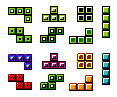
\includegraphics[width=\linewidth]{Team_logo_002.png}
		\caption{Liste des pi\`{e}ces utilis\'{e}es}
		\label{fig:sub2}
	\end{minipage}
	\begin{minipage}{.33\textwidth}
		\centering
		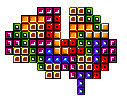
\includegraphics[width=\linewidth]{Team_logo_001.png}
		\caption{2\`{e}me version du logo}
		\label{fig:sub2}
	\end{minipage}
\end{figure}
\newpage
\begin{figure}[h!]
	\begin{minipage}{.5\textwidth}
		\centering
		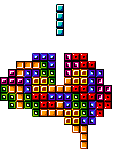
\includegraphics[width=0.75\linewidth]{Team_logo_004.png}
		\caption{Forme finale du logo}
		\label{fig:sub2}
	\end{minipage}
	\begin{minipage}{.5\textwidth}
		\centering
		
\includegraphics[width=0.75\linewidth]{Team_logo_005.png}
		\caption{Revision des pi\`{e}ces}
		\label{fig:sub2}
	\end{minipage}
\end{figure}

\begin{figure}[h!]
	\begin{minipage}{.5\textwidth}
		\centering
		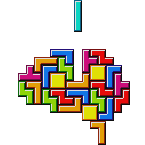
\includegraphics[width=0.75\linewidth]{Team_logo_007.png}
		\caption{R\'{e}vision des contour}
		\label{fig:sub2}
	\end{minipage}
	\begin{minipage}{.5\textwidth}
		\centering
		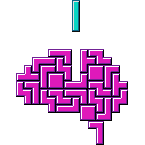
\includegraphics[width=0.75\linewidth]{Team_logo_008.png}
		\caption{Ajustement colorim\'{e}triques}
		\label{fig:sub2}
	\end{minipage}
\end{figure}

\newpage
			\section{Membres}

\begin{itemize}
\item Jean-François MIR
\item Charlotte JUDON
\item Ayoub BOUDEBIZA
\end{itemize}

	\part{Organisation}
	\setcounter{chapter}{0}
		\chapter{Organisation de l'\'{e}quipe de d\'{e}veloppement}
		\chapter{R\^{o}les et responsabilit\'{e}s}
	
	\part{Exigences}
	\setcounter{chapter}{0}
		\chapter{Crit\`{e}res pour valider une exigence}
			\section{Liste des crit\`{e}res}

\paragraph{Ci-dessous la liste restraintes des crit\`{e}res devant être valid\'{e}s pour qu'une nouvelle exigence soit analys\'{e}e:}
\begin{itemize}
\item R\'{e}tro / Pixel art style.
\item 8/16 bit (couleurs +  images/sprites).
\item M\'{e}canique et/ou \'{e}lectronique (pas d'organique).
\item Po\'{e}tique (implique peu / pas de texte à l'\'{e}cran).
\end{itemize}

		\chapter{Exigences majeures du projet}
			\section{Niveaux du jeu}

\paragraph{Les niveaux du jeu sont d\'{e}coup\'{e}s en 2 cat\'{e}gories : les niveaux projet\'{e}s par la machine et ceux dans le monde r\'{e}el.}

				\subsection{Niveaux projet\'{e}s par la machine}

\paragraph{Les niveaux projet\'{e}s par la machine permettent au jeune robot de pouvoir revivre les voyages de son ami à travers le monde et de faire avance le sc\'{e}nario (l’enquête). Il y a en tout 7 mondes à visiter:}

\begin{itemize}
\item P\'{e}kin (Chine).
\item Memphis (Egypte).
\item Rome (Italie).
\item Tenochtitlan (Mexique).
\item Atlantis (sous l’eau).
\item Pôle Nord (Pôle).
\item Crat\`{e}res (Lune).
\end{itemize}

\paragraph{Chacun de ces mondes est construit de la mani\`{e}re suivante :}

\begin{itemize}
\item 2 niveaux de plateforme classique.
\item 1 mini-boss de monde.
\item 2 niveaux de plateforme classique.
\item 1 boss de monde.
\end{itemize}

\paragraph{Les 2 premiers niveaux permettent au joueur de d\'{e}couvrir la m\'{e}canique principale du monde (par exemple : sauts contre les murs) et de la mettre à l’\'{e}preuve face à elle (par exemple : les ennemis peuvent sauter contre un mur ou de s’y accrocher. Le joueur ne peut pas le faire avant d’avoir vaincu le mini-boss. Les 2 niveaux suivants ainsi que le boss de monde mettent le joueur à l’\'{e}preuve avec cette m\'{e}canique (où il doit progresser avec ce nouveau pouvoir). Dans l’exemple cit\'{e}, le boss de monde fournirait alors le saut de mur infini.}

\paragraph{De mani\`{e}re g\'{e}n\'{e}rale, le mini-boss fournit la 1\`{e}re partie du pouvoir à d\'{e}bloquer. Le boss de monde fournit la seconde.}

				\subsection{Niveaux dans le monde r\'{e}el}

\paragraph{Les niveaux dans le monde r\'{e}el permettent de r\'{e}cup\'{e}rer les cartes postales. Le monde r\'{e}el prend place dans la ville natale du jeune robot et les cartes sont dispers\'{e}es dans les sous-sols du hangar.}

\paragraph{Le hangar est construit ainsi :}

\begin{itemize}
\item 6 directions à prendre au d\'{e}part.
\item 1 niveau puzzle dans chaque direction.
\item 1 boss puzzle à la fin de chaque niveau.
\end{itemize}

\paragraph{Le boss fourni la carte postale qui d\'{e}bloque l’acc\`{e}s à un monde.}

		\chapter{Exigences mineures du projet}
		\chapter{Historique des propositions d'exigences}


	\part{Recherche et d\'{e}veloppement}
	\setcounter{chapter}{0}
		\chapter{Game design}
		\chapter{Level design}
		\chapter{Chara design}
			\section{Robot (Joueur)}

\begin{figure}[h!]
	\caption{\label{Evol robot chara design} \'{e}volution du chara design du robot}
	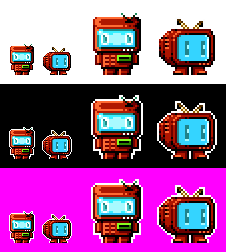
\includegraphics[scale=1]{Chara_design_001.png}
	\centering
\end{figure}

\begin{figure}[h!]
	\caption{\label{Color robot chara design} Tests de colorim\'{e}trie}
	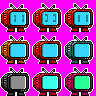
\includegraphics[scale=1]{Chara_design_002.png}
	\centering
\end{figure}

	\part{R\'{e}alisation}
	\setcounter{chapter}{0}
		\chapter{Processus}
		\chapter{Planning}
		
	\part{Suivi et contr\^{o}le}
	\setcounter{chapter}{0}

		\chapter{Environnement de d\'{e}veloppement}
			\section{Map Editor}
L'\'{e}diteur de niveau (minimap) se pr\'{e}sente de la manière suivante:
\begin{itemize}
\item Une image \'{e}ditable dont chaque pixel repr\'{e}sente un bloc de 32x32 pixel à l'\'{e}cran.
\item Un interpr\'{e}teur cod\'{e} en Python qui transcrit les couleurs des pixels en ID.
\item Un processus cod\'{e} en Python \'{e}galement qui contruit le sprite à partir de l'ID.
\end{itemize}

\begin{figure}[h!]
	\caption{\label{Minimap} Minimap (\'{e}diteur du niveau)}
	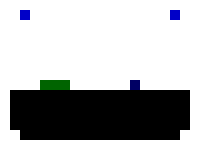
\includegraphics[scale=1]{minimap_002.png}
	\centering
\end{figure}

\begin{figure}[h!]
	\caption{\label{Minimap} Minimap (\'{e}diteur du niveau}
	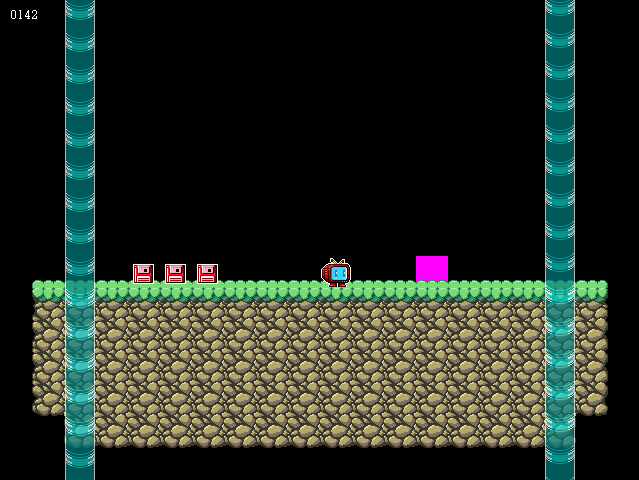
\includegraphics[scale=1]{map_001.png}
	\centering
\end{figure}

Les couleurs des pixels de la minimap codent donc les ID des blocs (sprites) de 32x32 pixels. La règle est la suivante:
\begin{itemize}
\item Chaque valeur R,G et B de la couleur du pixel repr\'{e}sente un bit de codage.
\item Les bits sont cod\'{e} en base 3 (valeurs possible par bit : 0, 1 ou 2).
\item les valeurs R, G et B sont multipli\'{e}es par 100 (0, 100 ou 200) afin de les diff\'{e}rencier lors de l'\'{e}dition
\item Exemple [R;G;B]: [0;200;100] devient [0;2;1]. L'ID = 0*9 + 2*3 +1*1 = 7.
\end{itemize}

		\chapter{Tests}
		\chapter{Optimisations}
			\section{Maitriser le nombre de sprites à l'\'{e}cran}
			
Les sprites sont le coeur même d'un jeu vid\'{e}o. Il est primordial de maitriser leur rafraichissement et leur nombre pour ne pas se retrouver avec de grosse perte
de FPS.

				\subsection{Version non optimis\'{e}e}
Initialement, le projet est programm\'{e} ainsi : Une grille sur laquelle viennent se poser des sprites (aka tiles) de collision :

\begin{figure}[h!]
	\caption{\label{Mapping initial des tiles} Mapping initial des tiles sur une grille}
	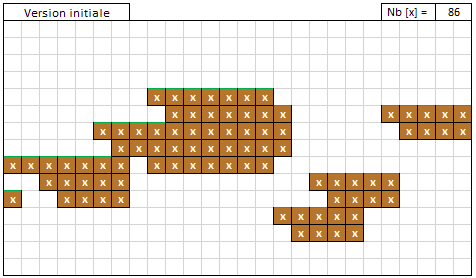
\includegraphics[scale=1]{Opti_tiles_001.png}
	\centering
\end{figure}
Sur cette 1\`{e}re vue on constate un grand nombre de tiles pour former les plateformes du jeu. Chaque tile n\'{e}cessite un rafraichissement à chaque frame pour
d\'{e}terminer si il se trouve à l'\'{e}cran ou non (afin de l'afficher et de le consid\'{e}rer dans la liste des tiles de collision actuel).

				\newpage
				\subsection{Propositions d'optimisations}

La r\'{e}duction de ces tiles en les regroupant permet d'acc\'{e}l\'{e}rer leur rafraichissement et de r\'{e}duire d'autant les check de collisions.
Ci-dessous sont pr\'{e}sent\'{e}es 3 m\'{e}thode distinctes qui d\'{e}taillent chacune le nombre de tiles restant ainsi que la part qu'elle repr\'{e}sente face au
mapping initial (le code couleur compare leur efficacit\'{e}):

\begin{figure}[h!]
	\caption{\label{Mapping opti 1} Mapping optimis\'{e} N°1}
	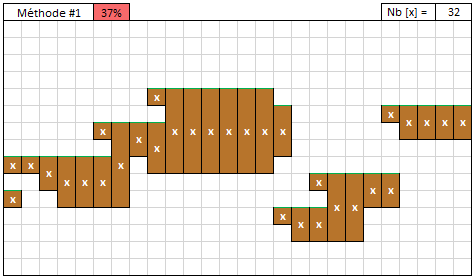
\includegraphics[scale=1]{Opti_tiles_002.png}
	\centering
\end{figure}
Chaque tile regroupe ici ceux \underline{verticalement adjactents}. Le nombre de tiles est divis\'{e} par 3 sur ce 1er essai. Il limite l'affichage de ceux
pr\'{e}sent dans l'\'{e}cran uniquement mais leur nombre augmentera lin\'{e}airement en fonction de la longueur du niveau à g\'{e}n\'{e}rer.

\begin{figure}[h!]
	\caption{\label{Mapping opti 2} Mapping optimis\'{e} N°2}
	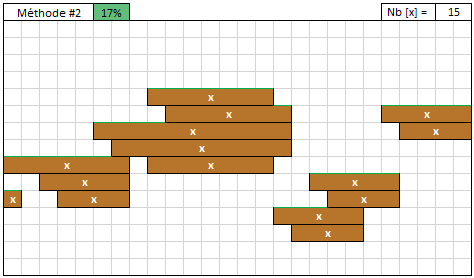
\includegraphics[scale=1]{Opti_tiles_003.png}
	\centering
\end{figure}
Chaque tile regroupe ici ceux \underline{horizontalement adjactents}. Le nombre de tiles est divis\'{e} par 6 sur ce 2\`{e}me essai. Il y a bien moins de tiles à
manipuler et rafraichir mais cela peut g\'{e}n\'{e}rer de tr\`{e}s long tiles (plus long que l'\'{e}cran) à maintenir afficher enti\`{e}rement.

\newpage

\begin{figure}[h!]
	\caption{\label{Mapping opti 3} Mapping optimis\'{e} N°3}
	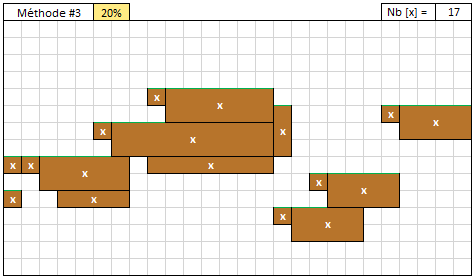
\includegraphics[scale=1]{Opti_tiles_004.png}
	\centering
\end{figure}
Chaque tile regroupe ici ceux \underline{verticalement et horizontalement adjactents}. Cette op\'{e}ration donne de bon r\'{e}sultats (similaire à la m\'{e}thode N2)
mais son impl\'{e}mentation semble difficile à r\'{e}aliser et maitriser.

				\subsection{Conclusion}
Suite au diff\'{e}rents tests r\'{e}alis\'{e}es, on peut synth\'{e}tiser les propositions ainsi:


\begin{tabular}{|l|c|c|l|l|}
\hline
Versions & Nb tiles & \% tile utilis\'{e}s & Int\'{e}rêts & Contraintes \\
\hline
Version initiale & 86 & 100\% & Impl\'{e}ment.n simple & Tr\`{e}s lourd à rafraichir \\
\hline
\hline
Group. vertical & 32 & 37\% & Aucun tile hors \'{e}cran & Pas efficace sur longs niveaux \\
\textbf{Group. horizontal} & \textbf{15} & \textbf{17\%} & \textbf{Tr\`{e}s peu de tiles} & \textbf{Tiles plus long que l'\'{e}cran} \\
Group. vert. + hor. & 17 & 20\% & Tr\`{e}s peu de tiles & Difficile à impl\'{e}menter \\
\hline
\end{tabular}


La proposition d'optimisation retenue est la seconde : \underline{Regroupement des tiles horizontalement}.

	\listoffigures

\end{document}